\chapter{Model Development}
\label{chap:model-dev}

\section{Data}

\subsection{UKCP Local and Met Office UK CPM}

\subsection{Precipitation}

* Coarsen to 8.8km (PSD plot?)
* 64x64 patch
* Differences between all 12 ensemble members
* Reducing skew
* Lack of correlation between CPM and GCM

\section{Methods}

\textcite{rampal2024mlclimdownscalingreview} find both nongenerative CNN approaches like U-Net \parencite{ronnenberger2015unet} and deep generative approaches to be effective in the domain on climate downscaling.

\subsection{U-Net}

Ronnenberger et al. and other uses in ML 4 weather and climate

\subsection{Diffusion}

Song et al.

\section{Inputs}

\subsection{Perfect vs imperfect}

\subsection{Avoid 925hPa}

\subsection{Feature selection}

\subsubsection{lr pr}

\subsubsection{V850}

Chan et al

\subsubsection{V4th}

\subsubsection{V4thT4th}

T for CCS

\subsubsection{V4thT4thS4th}

\subsubsection{pslV4thT4th}

\subsubsection{pslV4thT4thS4th}


\section{Training}

\subsection{Stabilizing validation loss}

The validation loss for a diffusion model can be unstable between epochs because the loss calculation involves both sampling from the noise scales and the initial noise distribution.
Therefore from epoch-to-epoch the validation loss can vary significantly (\autoref{fig:md:unstable-val-loss}) but without indicating a significant change in the model's performance, rather than some noise scales and initial noise samples are harder to get right than others.
This is also an issue for the training loss but in practice it is less of an issue.
Perhaps, because the larger training set size means there is less dependence on the noise scales and initial noise samples each epoch.
It would also be unwise to limit the choice of noise scales and initial noise samples in the same way when training as this could lead to poor performance on certain noise scales or initial noise samples that are not so well covered during training.
To solve this for the validation loss, I used the same samples of noise scales and initial noise for each epoch in order to ``stabilize'' the calculation and get loss curves that change more smoothly from epoch to epoch.
Another alternative would be a larger validation set.

Without the stochastic component this is issue does not affect the U-Net models.

\begin{figure}
  \centering
  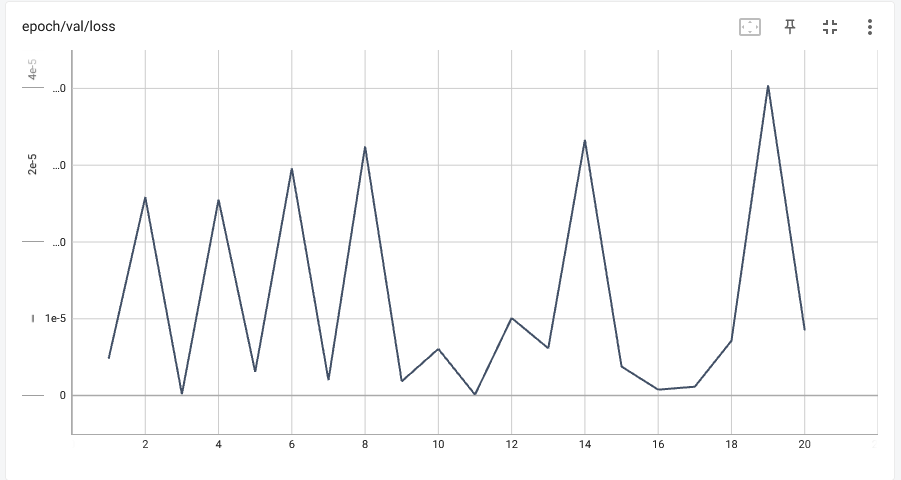
\includegraphics[width=\textwidth]{chapters/figures/3_md/loss/unstable-pr-12em-pslS4T4V4-val-loss.png}
  \caption{Unstable validation loss when different noise scales and initial noise samples are chosen at random each epoch}
  \label{fig:md:unstable-val-loss}
\end{figure}


\subsection{Stopping criteria}

With the validation loss stabilized, we can see when models start of overfit and select a checkpoint based on epochs where the validation loss is small.

With the reduced inputs and ensemble members, the 1em V850 model shows signs of overfitting once beyond the 100th-140th epoch, see \autoref{fig:md:loss}. The validation loss is unchanging between these epochs but clearly increasing again with more epochs.

\begin{figure}
  \centering
  \begin{subfigure}[b]{0.4\textwidth}
    \centering
    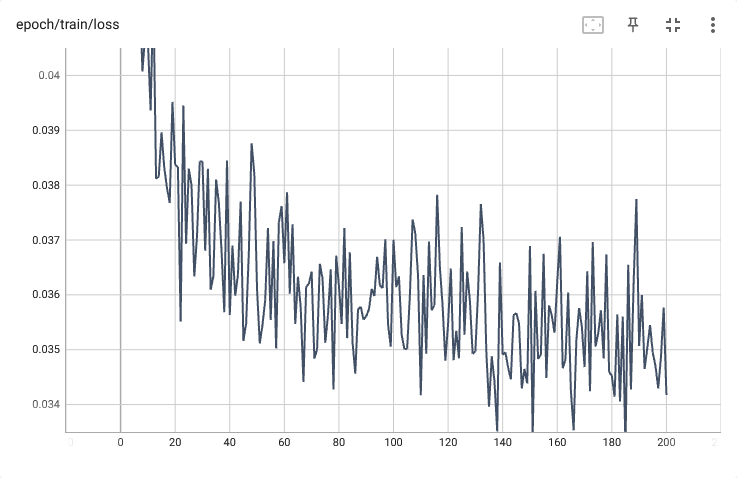
\includegraphics[width=\textwidth]{chapters/figures/3_md/loss/pr-1em-v850-train-loss.png}
      \caption{pr 1em v850 Train loss}
      \label{fig:md:1em-v850-train-loss}
  \end{subfigure}
  \hfill
  \begin{subfigure}[b]{0.4\textwidth}
      \centering
      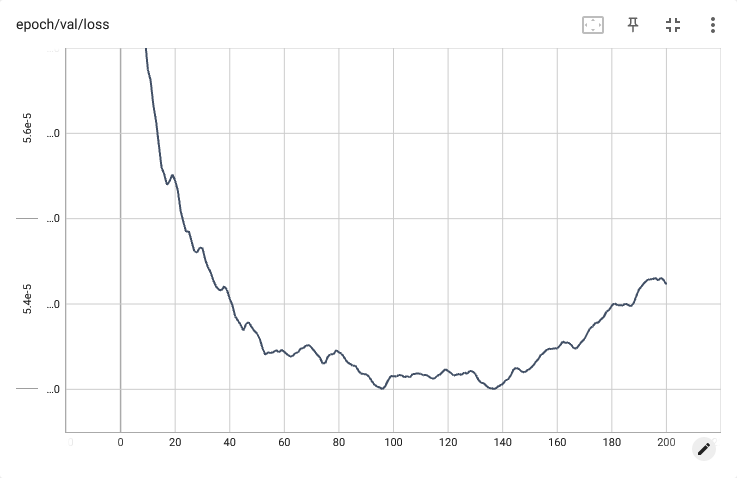
\includegraphics[width=\textwidth]{chapters/figures/3_md/loss/pr-1em-v850-val-loss.png}
      \caption{pr 1em v850 Val loss}
      \label{fig:md:1em-v850-val-loss}
  \end{subfigure}
  \hfill
  \caption{Train and validation loss for various iterations of the diffusion model.}
  \label{fig:md:loss}
\end{figure}

\section{Transfer to GCM inputs}